%%%%%%%%%%%%%%%%%%%%%%%%%%%%%%%%%%%%%%%%%%%%
% arara: pdflatex: { synctex: on }
% arara: pdflatex: { synctex: on }
\documentclass[oneside]{scrbook}

\usepackage[utf8]{inputenc}
\usepackage{polski}
%\usepackage{identfirst}
 \usepackage{amsfonts}
\usepackage{amsmath}
\usepackage{amsthm}
\usepackage{enumitem}   

\usepackage{graphicx}
\usepackage{caption}
\usepackage{tikz}
\usetikzlibrary{shapes.geometric, arrows}



\title{Języki formalne i złożoność obliczeniowa.}
\author{Na podstawie wykładu profesora Macieja Kandulskiego}
\date{semestr zimowy 2019/2020}


\titlehead{Notatki z wykładu Pani Sarenki}
\publishers{Uniwersytet Adama Mickiewicza wydział Matematyki i Informatyki}

\begin{document}
\maketitle

%\frontmatter
%\tableofcontents
%\listoffigures
%\listoftables

%\chapter{Acknowledgements}

%I would like to thank my supervisor, Professor Someone. This
%research was funded by the Imaginary Research Council.

%\chapter{Abstract}

%A brief summary of the project goes here.

%\mainmatter

\backmatter
\chapter{Wykład 12.10.2019}
\label{ch:wyklad1}

%%%%%%%%%%%%%%%%%%%%%%%%%%%%%%%%%%%%%%%%%%%%%%%%%%%%%%%%%%%%%%%%%%%%%%%%%%%%%%%%%%%%%%%%%
%%%%%%%%%%%%%%%%%%%%%%%%%%%%%%%%%%%%%%%%%%%%%%%%%%%%%%%%%%%%%%%%%%%%%%%%%%%%%%%%%%%%%%%%%
%%%%%%%%%%%%%%%%%%%%%%%%%%%%%%%%%%%%%%%%%%%%%%%%%%%%%%%%%%%%%%%%%%%%%%%%%%%%%%%%%%%%%%%%%
%%%%%%%%%%%%%%%%%%%%%%%%%%%%%%% Złożoność obliczeniowa %%%%%%%%%%%%%%%%%%%%%%%%%%%%%%%
\section{Złożoność obliczeniowa}

	Zagadnienia złożoności obliczeniowej
	- jakie są koszty prowadzenia obliczeń czasowe i pamięciowe:
	\begin{itemize}
	  \item Złożoność wykładnicza
	  \item Nierozsądne gospodarowanie czasem
	  \item Nierozsądne gospodarowanie pamięciową \ldots
	\end{itemize}

%%%%%%%%%%%%%%%%%%%%%%%%%%%%%%%%%%%%%%%%%%%%%%%%%%%%%%%%%%%%%%%%%%%%%%%%%%%%%%%%%%%%%%%%%
%%%%%%%%%%%%%%%%%%%%%%%%%%%%%%%%%%%%%%%%%%%%%%%%%%%%%%%%%%%%%%%%%%%%%%%%%%%%%%%%%%%%%%%%%
%%%%%%%%%%%%%%%%%%%%%%%%%%%%%%%%%%%%%%%%%%%%%%%%%%%%%%%%%%%%%%%%%%%%%%%%%%%%%%%%%%%%%%%%%
%%%%%%%%%%%%%%%%%%%%%%%%%%%%%%% Gramatyka %%%%%%%%%%%%%%%%%%%%%%%%%%%%%%%
\section{Gramatyka}

	\begin{mytheo}{Gramatyka}{theoexample}
		Jak poprawnie budować wyrażenia danego języka (zbiór zasad).
		Gramatyka inaczej jest nazywana syntaktyką albo składnią.
	\end{mytheo}
	
	
	%schemat gramatyki
	\begin{tikzpicture}
		\node[draw, rectangle, minimum width = 3 cm, minimum height = 2 cm] (fl) at (0,0) 
			{ \bf JĘZYK};
		% oznaczenie nad dgłównym prostokatem 
		%\node[above] at (fl.north) {$V(B)$};
		
		\draw[<-] (fl) -- node[above]{ \bf gramatyka} node[below]{generowanie wyrażeń} ++(-6,0);
		\draw[<-] (fl) -- node[above]{\bf automat} node[below]{rozpoznawanie wyrażeń tego języka} 
			++(8,0);
	\end{tikzpicture}
	
	Między innymi kompilator posiada w sobie element rozpoznający gramatykę. \newline

%%%%%%%%%%%%%%%%%%%%%%%%%%%%%%%%%%%%%%%%%%%%%%%%%%%%%%%%%%%%%%%%%%%%%%%%%%%%%%%%%%%%%%%%%
%%%%%%%%%%%%%%%%%%%%%%%%%%%%%%%%%%%%%%%%%%%%%%%%%%%%%%%%%%%%%%%%%%%%%%%%%%%%%%%%%%%%%%%%%
%%%%%%%%%%%%%%%%%%%%%%%%%%%%%%%%%%%%%%%%%%%%%%%%%%%%%%%%%%%%%%%%%%%%%%%%%%%%%%%%%%%%%%%%%
%%%%%%%%%%%%%%%%%%%%%%%%%%%%%%% Symbol %%%%%%%%%%%%%%%%%%%%%%%%%%%%%%%
\newpage
\section{Symbol a znaczenie symbolu}

	\subsection{Abstrakcyjne pojęcie liczby}
		
		Warto odróżnić symbol od jego znaczenia. Np. liczbę dwa można zapisywac w postaci symoblu 
		cyfry arabskiej { \bf 2} lub rzymskiej  { \bf II}. To samo dotyczy słowa 
		{ \bf słoń } - słowo oznacza wielkie kilkutonowe zwierze ale nim nie jest 
		(nie jest bytem materialnym). \newline

		 \begin{mytheo}{Abstrahować}{theoexample}
		 	Abstrahować znaczy pomijać. \newline
			Np.: abstrakcyjna liczba dwa powstała z pominięciem takich 
			cech jak wielkość, pochodzenie.
		\end{mytheo}

		 
	\subsection{Przykład powstania liczby}
		Różna materialne nośniki niosące te same liczby obiektów o różnych cechach. \newline
		Opisanie wspólnej cechy obiektów - { \bf liczebności} .
		
		\begin{enumerate}[label=(\roman*)]
		  \item {\bf couple} of people (para ludzi - 2)
		  \item {\bf pair} of pistols (para pistoletów - 2)
		  \item {\bf yoke} of oxen (zaprzęg dwa zwierzęta)
		\end{enumerate}
		 
		Abstrakcyjna liczba { \bf 2} powstała abstrahując od pochodzenia (np. zwierzęcia), 
		wielkości (np. broni) czy płci (para ludzi) pozostawiając tylko jedną wspólną cechę,
		którą jest { \bf liczebność} . 
		 

%%%%%%%%%%%%%%%%%%%%%%%%%%%%%%%%%%%%%%%%%%%%%%%%%%%%%%%%%%%%%%%%%%%%%%%%%%%%%%%%%%%%%%%%%
%%%%%%%%%%%%%%%%%%%%%%%%%%%%%%%%%%%%%%%%%%%%%%%%%%%%%%%%%%%%%%%%%%%%%%%%%%%%%%%%%%%%%%%%%
%%%%%%%%%%%%%%%%%%%%%%%%%%%%%%%%%%%%%%%%%%%%%%%%%%%%%%%%%%%%%%%%%%%%%%%%%%%%%%%%%%%%%%%%%
%%%%%%%%%%%%%%%%%%%%%%%%%%%%%%% języki formalne %%%%%%%%%%%%%%%%%%%%%%%%%%%%%%%
\newpage
\section{Języki formalne}
	\subsection{Pojęcia}
		
		Ciągi i zbiory ciągów traktowane są jako obiekty materialne a 
		{ \bf nie } abstrakycjne. \newline
		
		{ \bf Skończoność} - ważna cecha alfabetu/zbioru ponieważ tylko skończone 
		zbiory danych można przechowywać w { \bf fizycznym urządzeniu}. \newline \newline
		

		\begin{mytheo}{Alfabet V}{theoexample}
			Alfabet V to: { \bf dowolny} , { \bf niepusty} , 
			{ \bf skończony zbior znaków} \newline np.: V = \{I\} , V' = \{a,b\}. \newline
		\end{mytheo}


		\begin{mytheo}{Słowo nad alfabetem V}{theoexample}
			Słowo nad alfabetem V to dowolny, skończony ciąg znkaów z 
			V. np.: {\bf IIII} (słowo nad alfabetem V=\{I\}) czy {\bf abba} 
			(słowo nad alfabetem V=\{a,b\}) 
		\end{mytheo}


		\begin{mytheo}{Słowo puste $\epsilon$}{theoexample}
			Słowo puste $\epsilon$ - słowo o 0 (zerowym) wystąpieniu symboli. \newline
			Uwaga! Spacja {\bf NIE} jest słowem pustym.
		\end{mytheo}

		 
		 \begin{mytheo}{V*}{theoexample}
			Zbiór wszystkich słów nad alfabetem V. Łącznie z pustym słowem $\epsilon$.
		\end{mytheo}


		\begin{mytheo}{V* \textbackslash $ \{ \epsilon \}$ = V+}{theoexample}
			Zbiór wszsytkich niepustych słów. (Wyłączenie ze zbioru pustego słowa $\epsilon$)
		\end{mytheo}
		
		
		\begin{mytheo}{Oznaczenie słów}{theoexample}
			Słowa oznaczane są wielkimi literami z końca alfabetu łacińskiego, \newline
			np.: { \bf P},{\bf Q},{\bf R}. 
		\end{mytheo}
		

%%%%%%%%%%%%%%%%%%%%%%%%%%%%%%%%%%%%%%%%%%%%%%%%%%%%%%%%%%%%%%%%%%%%%%%%%%%%%%%%%%%%%%%%%
%%%%%%%%%%%%%%%%%%%%%%%%%%%%%%%%%%%%%%%%%%%%%%%%%%%%%%%%%%%%%%%%%%%%%%%%%%%%%%%%%%%%%%%%%
%%%%%%%%%%%%%%%%%%%%%%%%%%%%%%%%%%%%%%%%%%%%%%%%%%%%%%%%%%%%%%%%%%%%%%%%%%%%%%%%%%%%%%%%%
%%%%%%%%%%%%%%%%%%%%%%%%%%%%%%%%%%%%%%%%%%%%%%%%%%%%%%%%%%%%%%%%%%%%%%%%%%%%%%%%%%%%%%%%%%%%%
\newpage
\section{Konkatenacja}
	\subsection{Operacja konkatenacji}
	
		\begin{mytheo}{Konkatenacja dwóch słów}{theoexample}
			Konkatenacją dwóch słów {\bf P} i {\bf Q} nazywamy słowo {\bf PQ} 
			zdefiniowane w następujący sposób:
			
			\begin{enumerate}[label=(\roman*)]
				  \item jeżeli {\bf P}=$a_{1}, ... ,a_{n}$ gdzie 
				  {\bf a}=$b_{1}, ... ,b_{n}$ n,m $\ge$ 0 to 
				  {\bf PQ}= $a_{1},...,a_{n}b_{1},...,b_{n}$
				  
				  \item Jeżeli {\bf P}=$\epsilon$, to {\bf PQ}=Q.\newline 
				  Alternatywnie to {\bf Q}=$\epsilon$ i wtedy {\bf PQ}=P. \newline
				  Gdy {\bf P}={\bf Q}=$\epsilon$ to {\bf PQ=}$\epsilon\epsilon$ = $\epsilon$ . 
			\end{enumerate}

		\end{mytheo}

	
%%%%%%%%%%%%%%%%%%%%%%%%%%%%%%%
	
	\subsubsection{Własności konkatenacji}
		\begin{itemize}
		  \item Konkatenacja jest działaniem łacznym w zbiorze słów
		  
		  \item Konkatenacja w ogólnoście {\bf NIE} jest przemienna 
		  (bywa przemienna dla tyh samych słów {\bf ab} {\bf ab } ) lub 
		  jeśli alfabet skada sie tylko z jednego znaku np V = \{a\}
		  
		  \item $\epsilon$ słowo puste zachowje się jak element neutralny 
		  dla operacji konkatenacji: \newline $\epsilon$P $\subset$ P $\epsilon$ = P.
		\end{itemize}
	
%%%%%%%%%%%%%%%%%%%%%%%%%%%%%%%
	
	\subsection{Konkatenacja NIE jest grupą algebraiczną}
		Pomimo abstrakcyjnego znaczenia liczb, ich mentalna reprezentacja jest jednak w 
		urządzeniu czymś materialnym (stanami wysokich i niskich napięć).\newline \newline
		$V^{*}$ - zbiór wszystkich elementów (słów) nad alfabatem { \bf V} 
		(łącznie z elementem pustym $\epsilon$) \newline
		$\circ$ - oznacza działanie w grupie \newline				
		\textbf{e} - litera e jest symbolem elementu neutralnego \newline
		
		
		\begin{tcolorbox}
			\textbf{Przykład łączności:} \newline
			a) dodawanie np. : 2 + (3 + 5) = (2 + 3) + 5 \newline
			b) mnożenie np.:  2 * (3 * 5) = (2 * 3) * 5
		\end{tcolorbox}
		
		\begin{mytheo}{Warunki bycia grupą}{theoexample}

			Konkatenacja jest grupą (z algebry) jeśli spełnia warunki na bycie grupą:

			\begin{enumerate}[label=(\roman*)]
			  \item operacja $\circ$ jest łączna w grupie;
			  
			  \item $\exists e$, $\forall x $ Istnieje element neutralny dal każdego x, 
			  		taki że  $x \circ e = e \circ x = x$;
	
			  \item Dla każdego x $\forall x $   Istnieje element odwrotny  
				 $\exists x^{-1}$, taki, że  $x \circ  x^{-1} = x^{-1} \circ x = e$. 
				 \newline Warunek nie spełniony przez konkatenację - nie istnieje w 
				 ogólności takie słowo gdzie: słowo + słowo$^{-1} = \epsilon$
				 (szczególny przypadek spełnienia to $\epsilon$ + $\epsilon$ = $\epsilon$, 
				 bo element neutralny jest sam do siebie odwrotny $\epsilon^{-1} = \epsilon$ ) 
				 \newline $\Rightarrow$ 
				 {\bf WARUNEK NIE JEST W OGÓLNOŚCI SPEŁNIONY - konkatenacja NIE jest grupą!}
			\end{enumerate}

		\end{mytheo}

	
%%%%%%%%%%%%%%%%%%%%%%%%%%%%%%%
	
	\subsection{Podsłowo słowa}
		Zbiór { \bf A } $\subset$   { \bf A } i analogicznie  { \bf abca } $\sqsubset$  { \bf abca }
		(Znak $\sqsubset$  to taka kanciasta inkluzja oznaczenie używane przy słowach)
		
		\begin{mytheo}{Podsłowo}{theoexample}
			Mówimy, że słowo {\bf Q} jest podsłowem słowa {\bf P} wtedy i tylko wtedy gdy,
			istnieją słowa $Q_{1}$ i $Q_{2}$ takie, że:
			\begin{center}
			$P = Q_{1}${\bf Q}$Q_{2}$.
			\end{center}
			Np:. słowo {\bf bc} jest podsłowem słowa {\bf abcd} 
			
			\begin{center}
				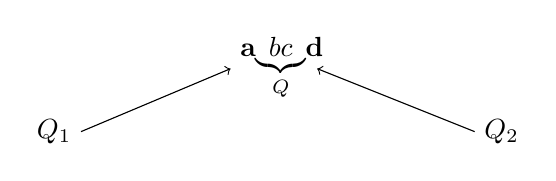
\begin{tikzpicture}
					\node[left]{$Q_{1}$};
					\draw[->] (0,0)-- (1.9,0.8) node[right]{{\bf a}$\underbrace{bc}_{Q}${\bf d}};
					\draw[<-] (3,0.8) -- (5,0) node[right]{$Q_{2}$};
				\end{tikzpicture}
			\end{center}
			
			Widać, tutaj, zę Q to słowo {\bf ab}, $Q_{1} = a$, $Q_{2}=d$
		\end{mytheo}
		
		 
		\begin{mytheo}{Prefix słowa}{theoexample}
			Słowo $Q$ jest prefixem słowa $P$ jeśli $P = QQ_{1}$.
		\end{mytheo}


 		\begin{mytheo}{Suffix słowa}{theoexample}
			Słowo $Q$ jest suffixem słowa $P$ jeśli $P =Q_{1}Q$.
		\end{mytheo}


 		\begin{mytheo}{Infix słowa}{theoexample}
			Słowo $Q$ jest infixem słowa $P$ jeśli $P =Q_{1}QQ_{2}$  \newline
			gdzie $Q_{1}\neq \epsilon$ i gdzie $Q_{2} \neq \epsilon$.		
		\end{mytheo}

	
%%%%%%%%%%%%%%%%%%%%%%%%%%%%%%%
	
	\subsection{Długość słowa}
		\begin{mytheo}{Długość słowa $\mid P\mid$ }{theoexample}
			Długością słowa $P \subset V^{*}$ nazywamy liczbę naturalną $\mid P\mid$ 
			definiujemy w sposób indukcyjny:
			 
			\begin{enumerate}[label=(\roman*)]
			  \item $ \mid  \epsilon \mid=0$
			  \item $ \mid P{ \bf a}  \mid= \mid P \mid + 1$; gdzie P to ciąg (słowo) a 
			  {\bf a} to symbol (dodatkowa litera w słowie).
			\end{enumerate} 
		\end{mytheo}
	
		
		\begin{tcolorbox}
			\textbf{Przykład 1.: } Długość słowa {\bf abc} \newline
			$\mid abc \mid = \mid ab \mid + 1 = ( \mid a \mid + 1) + 1 = 
			(\mid \epsilon a \mid + 1) + 1 =   ((\mid \epsilon \mid + 1 )+1)+1 =
			((0+1)+1)+1 = 3$
	
		\end{tcolorbox}
		
		
		\begin{tcolorbox}
			\textbf{Przykład 2.: } \newline 
			Obliczyć ilość wszystkich podsłów słowa  
			\textbf{P} gdy dana jest długość słowa $\mid P \mid = 4$ \newline 
			
			\textbf{Odp: NIE WIĘCEJ NIŻ} 11. \newline \newline

			\textbf{Rozwiązanie a:}\newline
			Weźmy dla przykładu słowo {\bf abcd }. 
			
			Podsłowo {\bf abcd} $\subset$ {\bf abcd} - jedno podsłowo długości 4. 
			(Słowo jest samo swoim podsłowem; kolejnosć znaków też ma znaczenie np słowo 
			{\bf bcda} $\not\subset $ {\bf abcd}  ).
			\newline
			
			Podsłowa długości 3 (2 takie słowa)
			{\bf abc} $\subset$ {\bf abcd},
			{\bf bcd} $\subset$ {\bf abcd};
			
			Podsłowa długości 3 (2 takie słowa)
			{\bf ab} $\subset$ {\bf abcd},
			{\bf bc} $\subset$ {\bf abcd},
			{\bf cd} $\subset$ {\bf abcd};
			
			Podsłowa długości 1 (4 takie słowa)
			{\bf a} $\subset$ {\bf abcd},
			{\bf b} $\subset$ {\bf abcd},
			{\bf c} $\subset$ {\bf abcd},
			{\bf d} $\subset$ {\bf abcd}; \newline
							
			\textbf{Odp a:} \newline
			Dla słowa \textbf{abcd} mamy (1+2+3+4) + 1 \newline
			( dodajemy jeden bo znak pusty $\epsilon$ ) \newline
			
			------------------------------------------------------------------------------\newline
			
			\textbf{Rozwiązanie b):} \newline
			Załóżmy, że szukamy wszystkich podsłów słowa P = {\bf aaaa}. \newline
			aaaa $\subset$  aaaa (1 podsłowo) \newline
			aaa $\subset$  aaaa (1 podsłowo) \newline
			aa $\subset$  aaaa (1 podsłowo) \newline
			a $\subset$  aaaa (1 podsłowo)  \newline
			
			\textbf{Odp b:} \newline
			Dla słowa { \bf aaaa} mamy (1+1+1+1) + 1 (dodajemy jeden bo znak 
			pusty $\epsilon$ ).\newline 
			 \textbf{NIE ROZRÓŻNIAMY ZNAKÓW MIĘDZY SOBĄ tzn.: zawsze a == a} 
			(nie rozróżniamy permutacji tych samych elementów)
			
		\end{tcolorbox}
	
		
		%%%%%%%%%%%%%%%%%%%%%%%%%%%%%%% Zadanie domowe 12.10.2019 %%%%%%%%%%%%%%%%%%%%%%%%%%%%%%%
		
		\begin{tcolorbox}
			\textbf{Zadanie Domowe 12.10.2019} \newline
			
			Napisać procedurę w pseudokodzie:
			Dla zadanego słowa długośc {\bf n} napisac procedurę, które pokaże liczbę {\bf k}
			podsłów oraz wypisze całą listę konkretnych podsłów.
		\end{tcolorbox}
		
		%%%%%%%%%%%%%%%%%%%%%%%%%%%%%%% Rozwiazanie %%%%%%%%%%%%%%%%%%%%%%%%%%%%%%%
		\begin{lstlisting}
		
		
		Tu bedzie rozwiazanie:
		    if (n == 0 || n == 1){    
		      return n;        
		    }        
		    j = 0;    
		    for (i = 0; i < n-1; i++){      
		      if (arr[i] != arr[i+1]){        
		        arr[j] = arr[i];       
		        j++;      
		      }       
		    }      
		    arr[j++] = arr[n-1];
		\end{lstlisting}
	
	%%%%%%%%%%%%%%%%%%%%%%%%%%%%%%% Długość konktatenacji słów %%%%%%%%%%%%%%%%%%%%%%%%%%%%%%%
	
	
	\subsection{Długość konkatenacji słów}
		\begin{mytheo}{Długość konktatenacji słów}{theoexample}
	
			\begin{center}
			$\mid PQ \mid = \mid P \mid + \mid Q \mid$
			\end{center}
			
			Dowód (indukcja matematyczna):\newline
			$\forall P,Q: \mid PQ \mid = \mid P \mid + \mid Q \mid$ 
			(Indukcja po długości $\mid Q \mid$)
			
			\begin{enumerate}[label=(\roman*)]
				\item $\mid Q \mid = \epsilon$ \newline
				LewaStrona: $\mid PQ \mid = \mid P \epsilon \mid = \mid P \mid$ gdzie 
				k $ \leq $ n \newline
				PrawaStrona: $\mid P \mid + \mid Q \mid = 
				\mid P \mid + \mid \epsilon \mid = 
				\mid P \mid+ 0 = \mid P \mid $ = { \bf LewaStrona} c.d.n \newline
				  
				  
				\item  $\lambda$: $\mid PQ \mid = \mid P \mid + \mid Q \mid $ \newline
				PrawaStrona: $\mid P(Qa) \mid = \mid P \mid  + \mid Qa \mid$  gdzie n=0\newline
				LewaStrona: $ \mid P(Qa) \mid \overset{\mathrm{jeżeli}}{=} 
				\mid (PQ)a \mid \overset{\mathrm{ii}}{=} 
				\mid PQ \mid + 1 \overset{\mathrm{\lambda}}{=}$ \newline
				$(\mid P \mid + \mid Q \mid) + 1 = 
				\mid P \mid + (\mid Q \mid + 1) = 
				\mid P \mid + \mid Qa \mid$ ,..., = { \bf  PrawaStrona } c.n.d
			
			\end{enumerate} 
		\end{mytheo}

%%%%%%%%%%%%%%%%%%%%%%%%%%%%%%% N-ta potęga słowa %%%%%%%%%%%%%%%%%%%%%%%%%%%%%%%
	
	\subsection{N-ta potęga słowa}
		Przykład potęgowania liczb: \textbf{$ \underbrace{7*7* ... *7}_{n-razy} = 7^{n}$}\newline
		Potęgowanie słów: \textbf{abcabcabc} = $(abc)^{3} /neq a^{3}b^{3}c^{3}$
		
		\begin{mytheo}{N-ta potęga liczby}{theoexample}
			Potęgowanie liczb - widać że pierwszy warunek $a^{0} = 1$ jest stworzony przez
			 matematyków, niejako sztucznie ale jest to wymagane dla prawdiłowości działania
			 indukcji matematycznej; a w praktyce jest to często warunek zatrzymania funkcji
			 obliczającej np. silnie iteracyjnie czy rekurencyjnie.
		
			\begin{enumerate}[label=(\roman*)]
				\item $a^{0} = 1$
				
				\item $a^{n+1} = a^{0+1}=a^{0}*a$
			\end{enumerate} 
		\end{mytheo}
	
	
		Podobnie jak liczby potęguje się też słowa, ale ze względu na swoją specyfikę
		kolejność znaków w słowie podczas mnożenia ma znaczenie!
	
		\begin{mytheo}{N-ta potęga słowa}{theoexample}
			N-tą potęgą słowa \textbf{P}, oznaczamy \textbf{$P^{n}$}, nazywamy słowo 
			zdefiniowane indukcyjnie w następujący sposób:
		
			\begin{enumerate}[label=(\roman*)]
				\item $P^{0} = \epsilon$
				\item $P^{n+1} = P^{n}P$
			\end{enumerate} 
					
			Dowód:
			$\underbrace{P^{1}}_{}= P^{0+1} \overset{\mathrm{ii}}{=}  P^{0}\underbrace{P}$		

		\end{mytheo}
		
		\begin{tcolorbox}
			\textbf{Przykład:} \newline
			$a^{3}(ba)^{2}= aaababa$ \newline
			$(abc)^{3} \neq a^{3}b^{3}c^{3}$
		\end{tcolorbox}
	
	
%%%%%%%%%%%%%%%%%%%%%%%%%%%%%%% Rewers %%%%%%%%%%%%%%%%%%%%%%%%%%%%%%%
	
	\subsection{Operacja Odbicia zwierciadlanego (rewers) słowa P}
		Przykład odbicia zwierciadlanego to po prostu pisanie wyrazu "od tyłu" \newline
		np.: $(abc)^{-1}$ = cba \newline
				
		\begin{mytheo}{Odbicie zwierciadlane słowa P}{theoexample}
			Odbicie zwierciadlane słowa \textbf{P}, oznaczamy przez $P^{-1}$ 
			(P prim)i definiujemy je indukcyjnie po $\mid P \mid '$ w następujący sposób:
		
			\begin{enumerate}[label=(\roman*)]
				\item $\epsilon^{-1} = \epsilon$
				\item $(Pa)^{-1} = aP^{-1}$  //odwróciliśmy a teraz odwracamy resztę słowa 			
						\textbf{P}
			\end{enumerate} 
		
		\end{mytheo}

%%%%%%%%%%%%%%%%%%%%%%%%%%%%%%% Własności konkatenacji %%%%%%%%%%%%%%%%%%%%%%%%%%%%%%%
	
	\subsection{Własności konkatenacji}
		\subsubsection{Rewers Konkatenacji (odbicie zwierciadlane)}
			$(PQ)^{-1} = Q^{-1}P^{-1}$
	
		\subsubsection{Rewers N-tej potęgi konkatenacji}
			$(P^{n})^{-1} = (P^{-1})^{n}$  np.: $((abc)^{3})^{-1} = (cba)^{3}$
		
		\subsubsection{Złożenia odbić zwierciadlanych konkatenacji}
			$(P^{-1})^{-1} = P$ //odbicia znoszą się


%%%%%%%%%%%%%%%%%%%%%%%%%%%%%%%%%%%%%%%%%%%%%%%%%%%%%%%%%%%%%%%%%%%%%%%%%%%%%%%%%%%%%%%%%
%%%%%%%%%%%%%%%%%%%%%%%%%%%%%%%%%%%%%%%%%%%%%%%%%%%%%%%%%%%%%%%%%%%%%%%%%%%%%%%%%%%%%%%%%
%%%%%%%%%%%%%%%%%%%%%%%%%%%%%%%%%%%%%%%%%%%%%%%%%%%%%%%%%%%%%%%%%%%%%%%%%%%%%%%%%%%%%%%%%

\newpage
\section{Język}
	\begin{mytheo}{Alfabet a język}{theoexample}
		Uwaga - alfabet V $\not\Leftrightarrow$ język. \newline
	\end{mytheo}

	Należy takze pamiętać, że:
	 $V^{*}$ - zbiór wszystkich elementow (słów) nad alfabatem 
	 { \bf V} (łącznie z elementem pustym $\epsilon$)\newline \newline
	
	%schemat gramatyki
	\begin{tikzpicture}
		\node[draw, rectangle, minimum width = 3 cm, minimum height = 2 cm] (fl) at (0,0) 
		{ \bf JĘZYK};
		
		% oznaczenie nad dgłównym prostokatem 
		%\node[above] at (fl.north) {$V(B)$};
		
		\draw[<-] (fl) -- node[above]{ \bf generator}  ++(-6,0);
		\draw[<-] (fl) -- node[above]{\bf rozpoznawanie} ++(8,0);
	\end{tikzpicture}\newline
	
	Przykładowo mamy \textbf{język angielski} składający się z małych liter \textbf{V=\{a,b,...z\}}
	Słowo \textbf{cat} należy do tego języka  tzn.: \textbf{ cat $\subset$ jezykAngielki}; \newline 
	a słowo \textbf{kot} chociaż jego znaki należą do alfabetu \textbf{V} to jednak słowo
	\textbf{"kot"} nie należy do \textbf{języka angielkiego} tzn.: \textbf{kot $\not\subset$
	językAngielski}.
	
	%%%%%%%%%%%%% rysunek zbioru %%%%%%%%%%%%%
	\begin{center}
		\begin{tikzpicture}
			\draw (0,0) rectangle (8,5);  
			\node [at={(1,4)}] {$V^{*}$};
			\draw[pattern=north east lines, pattern color=light-gray ] 
					(4.5,2) ellipse[x radius = 3, y radius = 1.5];
			\node [at={(2.5,1.5)}] {kot};
			\draw [fill, color=black] (2.5,1.7) circle(0.05cm); %punkt
			\draw [fill, color=white] (5,2) ellipse [x radius =2, 
			y radius = 1];
			\node [at = {(5,2)}] {$cat$};
			\draw [fill, color=black] (5,2.2) circle(0.05cm); %punkt
	
		\end{tikzpicture}
	\end{center}
	
	\begin{mytheo}{Język}{theoexample}
		Językiem nad alfabetem \textbf{V} nazywamy dowolny podzbiór zbioru wszystkich słów nad
		 \textbf{V} tj.:
		\begin{center}
			L $\subset V^{*}$ 
		\end{center}
	\end{mytheo}
	
	\begin{tcolorbox}
		\textbf{Przykład} \newline
		Dany jest alfabet binary V=\{0,1\}, czyli, żeby zaprezenetować wszystie liczby
		parzyste większe od 0 nalezy na ostatnim bicie umieścić cyfrę 0.
		
		%%%%%%%%%%%%% rysunek zbioru liczby binarne %%%%%%%%%%%%%
		\begin{center}
			\begin{tikzpicture}
				\draw[pattern=north east lines, pattern color=light-gray ] 
						(4, 4) circle(2.3cm);
				\node [at={(3,5)}] {V*};
				\draw [fill, color=white] (5,3) circle(0.7cm);
				\node [at = {(5,3)}] {1,..,0};
			\end{tikzpicture}
		\end{center}
		
	\end{tcolorbox}
	
	%%%%%%%%%%%%%%%%%%%%%%%%% Język jako zbiór  %%%%%%%%%%%%%%%%%%%%%%%%%
	\subsection{Język jako zbiór - własności}
		Jako obiekt język to zbiór $\rightarrow$ dziedziczy wszystkie własności zbioru:
		
		\begin{itemize}
		  \item A $\subset$ A
		  \item $V^{*} \subset V^{*}$
		  \item $\O \subset$ A
		  \item $\O \subset V^{*}$
		\end{itemize}
		
		
		\begin{tcolorbox}
			\textbf{Przykład} \newline
			%%%%%%%%%%%%% zbiory %%%%%%%%%%%%%
			\begin{center}
				\begin{tikzpicture}
					\draw[pattern=north east lines, pattern color=light-gray ] 
							(4, 4) circle(2.3cm);
					\node [at={(3,5)}] {V*};
					\draw [fill, color=white] (4,3) circle(1.2cm);
					\node [at = {(4,3)}] {L1};
				\end{tikzpicture}
			\end{center}
		
			Przykładowe operacje
			\begin{itemize}
			  \item $L_{1}, L_{2} \subset$ $V^{*}$
			  \item $L_{1} \cup L_{2}$
			  \item $L_{1} \cap L_{2}$
			  \item $L_{1} \setminus L{2}$
			  \item $\overline{L_{1}} = V^{*} \setminus L_{1}$
			\end{itemize}
		\end{tcolorbox}
	
	
	%%%%%%%%%%%%%%%%%%%%%%%%% Konkatenacja języków  %%%%%%%%%%%%%%%%%%%%%%%%%
	\subsection{Konkatenacja języków}
		\begin{mytheo}{Konkatenacja języków}{theoexample}
			Dla języków $L_{1}$ i $L_{2}$ przez konkatenację tych języków, 
			oznaczoną $L_{1}L_{2}$ rozumiemy zbiór:=
			\begin{center}
				$L_{1}L_{2} =\{P_{1}P{2}: P_{1} \in L_{1}, P_{2} \in L_{2}\}$
			\end{center}
		\end{mytheo}
		
		
		\begin{tcolorbox}
			\textbf{Przykład 1} \newline
			Mając języki  $L_{1}=\{a, ab, \epsilon \}$, $L_{2}=\{ b,ab, ba \}$.\newline
			Ile możemy utworzyć słów poprzez konkatenację języków $L_{1}$ i $L_{2}$? \newline
			\textbf{Odp: Maksymalnie 9.} \newline
			Rozwiązanie (najlepiej takie rzeczy robić tabelką):\newline
				\begin{tabular}{|l||*{5}{c|}}\hline
					\backslashbox{$L_{1}$}{$L_{2}$}
					&\makebox[3em]{b}&\makebox[3em]{ab}&\makebox[3em]{ba}
					\\\hline\hline
					a  			& ab		& $a^{2}b$		& $ba^{2}$ 		\\\hline
					ab 			& $ab^{2}$ 	& $(ab)^{2}$	& $ab^{2}a$ 	\\\hline
					$\epsilon$ 	& b			& ab			& ba			\\\hline
				\end{tabular}\newline
			Tabelka jest idealnym sposobem liczenia konkatenacji języków. \newline
			{\color{red} Uwaga przy konkatenacji trzeba uważać, czy pytanie dotyczyło 
			wszystkich możliwych kombinacji( wtedy liczymy z powtórzeniami), czy tylko 
			unikatowych słów.} \newline
		\end{tcolorbox}
		
	
		\begin{tcolorbox}
			\textbf{Przykład 2} \newline
			Mając języki: \newline 
				$L_{1}= \{ \epsilon, a, a^{2}, a^{3}, a^{4}, ... \} = {a^{n}: n \ge 0}$ \newline
				$L_{2}= \{ \epsilon, b, b^{2}, b^{3}, b^{4}, ... \} = {b^{n}: n \ge 0}$ \newline
		
			Odp:
				$L_{1}L_{2} = \{ a^{n}b^{m}: n,m \ge 0 \}$	// n,m $\ge$ 0 bo dopuszczamy $		 
				\epsilon * \epsilon$ równy 0
				
		\end{tcolorbox}
		
		
		\begin{tcolorbox}
			\textbf{Przykład 3} \newline
			Konkatenacja niepustego alfabetu ze sobą samym: \newline 
				Np.: L = $\{ a,b \}$ \newline
				Odp: LL = $\{a, b\}\{a, b\} = \{a^{2}, ab, ba, b^{2}\}$
		\end{tcolorbox}
		
		\begin{tcolorbox}
			\textbf{Przykład 4} \newline
			Konkatenacja alfabetu mającego tylko puste słowo ze sobą samym: \newline
			{\color{red} Uwaga  zbiór pusty $\O \neq \{ \epsilon \}$.} \newline
				Np.: L = $\{ \epsilon \}$
				Odp: LL = $\{ \epsilon \}\{ \epsilon \} = \{ \epsilon \}$
		\end{tcolorbox}
		
		\begin{tcolorbox}
			\textbf{Przykład 5} \newline
			Konkatenacja alfabetu posiadającego element pusty ze sobą samym: \newline 
				Np.: L = $\{ \epsilon , a, a^{2}, a^{3}, ... \} =  \{a^{n}: n \ge 0 \}$ \newline
				Odp: LL = $ \{ a^{n}: n \ge 0  \} \{ a^{n}: n \ge 0 \} = \{ a^{n}: n \ge 0 \}$
		\end{tcolorbox}
	
	
	%%%%%%%%%%%%%%%%%%%%%%%%% Potęga języków  %%%%%%%%%%%%%%%%%%%%%%%%%
	\subsection{Potęga języka}
	
	
	\begin{mytheo}{N-ta potęga języka}{theoexample}
		N-tą potęgą języka \textbf{L} nazywać będziemy język \textbf{$L^{n}$} zdefiniowany indukcyjnie w 	
		następujący sposób: 
	
		\begin{enumerate}[label=(\roman*)]
			\item $L^{0}={\epsilon}$
			\item $L^{n+1}=L^{n}L$
		\end{enumerate} 
	
	\end{mytheo}
	
	
	\begin{tcolorbox}
		\textbf{Zadanie:} \newline
			Pokazać że: $L^{1} = L$.
	\end{tcolorbox}
	
	
	\subsubsection{Konkatenacja zbiorów}
		\begin{mytheo}{Konkatenacje ze zbiorem pustym}{theoexample}
			Konkatenacja zbioru ze zbiorem pustym daje zbiór pusty: \newline
			$L\O = \{ P_{1}P_{2} : P_{1} \in L, P_{2} \in \O \} = \O$
		\end{mytheo}
		
		\begin{mytheo}{Konkatenacje ze zbiorem mającym tylko element pusty}{theoexample}
			Konkatenacja zbioru ze zbiorem mającym tylko element pusty: \newline
			$L \{ \epsilon \} = \{ P_{1}P_{2}: P_{1} \in L_{1}, P_{2} \in \{ \epsilon \} \} = 
			\{ P_{1}\epsilon : P_{1} \in L \} = \{ P_{1} : P_{1} \in L \} = L$
		\end{mytheo}
		

		\begin{tcolorbox}
			\textbf{Zadanie:} \newline
			Słowo  \textbf{P} należy do trzeciej potęgi języka \textbf{L}, $P \in L^{3}$ 
			wtedy i tylko wtedy gdy 
			
				\begin{center}
					$P=P_{1}P_{2}P_{3}$ :  $P_{1},P_{2},P_{3} \in L$
				\end{center}
						
			\textbf{Rozwiązanie:} \newline
			Niejednoznacze, bo P składa się z trzech słów, ale słowo $P_{n}$ 
			nie musi być jednoliterowe. \newline
			
			Przykładowo weźmy język L = $\{ a^{n} : n \ge 0\}$ \newline
			np.: $a^{5} \in L^{5}$ czyli $P_{1}P{2}P{3} \Leftrightarrow a*a*a^{3}$ \newline \newline
			
			$L^{0} = \{ \epsilon \}$ \newline
			$L^{1} = L = \{ a \}$ \newline
			$L^{2} = \{ a^{2} \}$ \newline
			$L^{3} = \{ a^{3} \}$ \newline
			$L^{4} = \{ a^{4} \}$ \newline
			$L^{5} = \{ a^{5} \}$ \newline \newline
			
			Teraz dodajemy znak pusty $\epsilon$ do języka L: \newline
			L = $\{\epsilon, a\}$ \newline
			$L^{1} = L = \{ \epsilon, a \}$ \newline
			$L_{2} = {a^{2}, a}$ \newline
			
			\begin{center}
				---------------- Na tym skończył się wykład 12.10.2019 ----------------
			\end{center}
		
		\end{tcolorbox}


%\backmatter

\end{document} 